% !TeX root = ../main.tex
% Supplementary material relocated from ch3/papers/exp_vocab/main.tex.
\chapter[Supplementary materials for Chapter 3]{Supplementary materials for Chapter 3: corpus-CDI}
\label{app:vocabulary}
\begingroup
\graphicspath{{ch3/papers/exp_vocab/}}
\providecommand{\meCDI}{\textsc{corpus-CDI}}


\section{Training and generation details}

Table~\ref{tab:train} summarizes the age-appropriate scaling of training data across three exposure scenarios. Linguistic exposure estimates are based on daylong recording studies \citep{cristia2019child}, which document substantial variability in the amount of speech heard by children across environments. Annual exposure ranges from approximately 100 hours in low-input households to 1000 hours in high-input ones, with 500 hours per year representing a mid-range estimate.

Cumulative exposure thus increases from 50–500 hours at 6 months to 300–3000 hours by 36 months. The reported word budgets range from 0.58M words (6 months, low exposure) to 34.71M words (36 months, high exposure).


\begin{table}[ht]
\centering
\small
\begin{tabular}{l c c c c}
\toprule
\textbf{Age (mo.)} & \textbf{Hours} & \textbf{Words (M)} & \textbf{Chars. (M)} & \textbf{Utts. (k)} \\

\midrule
\multicolumn{5}{l}{\textit{Low exposure scenario (100 hours/year)}} \\
\midrule
6   & 50   & 0.58  & 2.95  & 58   \\
12  & 100  & 1.16  & 5.89  & 116  \\
18  & 150  & 1.73  & 8.84  & 173  \\
24  & 200  & 2.31  & 11.78 & 231  \\
30  & 250  & 2.89  & 14.73 & 289  \\
36  & 300  & 3.47  & 17.67 & 347  \\
\midrule
\multicolumn{5}{l}{\textit{Medium exposure scenario (500 hours/year)}} \\
\midrule
6   & 250  & 2.89  & 14.73 & 289  \\
12  & 500  & 5.78  & 29.45 & 578  \\
18  & 750  & 8.68  & 44.18 & 868  \\
24  & 1000 & 11.57 & 58.90 & 1157 \\
30  & 1250 & 14.46 & 73.63 & 1446 \\
36  & 1500 & 17.35 & 88.35 & 1735 \\
\midrule
\multicolumn{5}{l}{\textit{High exposure scenario (1000 hours/year)}} \\
\midrule
6   & 500  & 5.78  & 29.45 & 578  \\
12  & 1000 & 11.57 & 58.90 & 1157 \\
18  & 1500 & 17.35 & 88.35 & 1735 \\
24  & 2000 & 23.14 & 117.80 & 2314 \\
30  & 2500 & 28.92 & 147.25 & 2892 \\
36  & 3000 & 34.71 & 176.70 & 3471 \\
\bottomrule
\end{tabular}
\caption{\textbf{Age-appropriate scaling of training datasets across three exposure scenarios.} Estimates are derived from three exposure scenarios (100h, 500h, 1000h per year), reflecting observed variability in children’s linguistic environments \citep{cristia2019child}. Word budgets are reported in millions, character counts in millions, and utterance counts in thousands. Character counts use 5.1 characters/word and utterance counts use 10 words/utterance. The hours-to-words conversion requires reconciliation with the training records, as noted in the main methods.}
\label{tab:train}
\end{table}


Table~\ref{tab:model} records the reported optimization and architecture settings. The prose describes the Transformer dimension as a hidden-state size, whereas the table labels it as an intermediate dimension; the run configuration is needed to resolve that distinction.


\begin{table}[ht]
\centering
\begin{tabular}{@{} l l @{}}
\hline
\textbf{Hyperparameter} & \textbf{Value} \\
\hline
Max sequence length & 1024 \\
Batch size & 64 \\
Learning rate & 0.0001 \\
Learning rate scheduler & inverse sqrt \\
Warmup steps & 10000 \\
Optimizer & Adam \\
Adam-beta1 & 0.9 \\
Adam-beta2 & 0.98 \\
Dropout & 0.1 \\
\hline
\textbf{LSTM hyperparameter} & \textbf{Value} \\
\hline
decoder layers & 3 \\
hidden size & 1024 \\
embedding dimension & 200 \\
\hline
\textbf{Transformer hyperparameter} & \textbf{Value} \\
\hline
Transformer layers & 12 \\
Intermediate hidden size & 512 \\
Attention heads & 12 \\
Attention dropout & 0.05 \\
\hline
\end{tabular}
\caption{\textbf{Language model training hyperparameters.} Reported optimization and architecture settings; the Transformer dimension label requires verification against the run configuration.}
\label{tab:model}
\end{table}


\begin{table}[!h]
\centering
\begin{tabular}{rrrr}
\toprule
\textbf{month} & \textbf{\#sec/hour} & \textbf{estimation} & \textbf{production} \\
\midrule
6 & 61.25 & 55,125 & 782 \\
7 & 65.30 & 58,769 & 1,323 \\
8 & 69.35 & 62,412 & 1,278 \\
9 & 73.40 & 66,056 & 3,964 \\
10 & 77.44 & 69,699 & 627 \\
11 & 81.49 & 73,343 & 1,148 \\
12 & 85.54 & 76,986 & 1,361 \\
13 & 89.59 & 80,630 & 568 \\
14 & 93.64 & 84,273 & 2,720 \\
15 & 97.69 & 87,917 & 13,765 \\
16 & 101.73 & 91,560 & 3,620 \\
17 & 105.78 & 95,204 & 7,589 \\
18 & 109.83 & 98,847 & 15,197 \\
19 & 113.88 & 102,491 & 17,090 \\
20 & 117.93 & 106,134 & 19,912 \\
21 & 121.98 & 109,778 & 33,458 \\
22 & 126.02 & 113,421 & 33,880 \\
23 & 130.07 & 117,065 & 63,738 \\
24 & 134.12 & 120,708 & 191,062 \\
25 & 138.17 & 124,352 & 130,525 \\
26 & 142.22 & 127,995 & 136,195 \\
27 & 146.27 & 131,639 & 148,741 \\
28 & 150.31 & 135,282 & 158,910 \\
29 & 154.36 & 138,926 & 190,263 \\
30 & 158.41 & 142,569 & 195,549 \\
31 & 162.46 & 146,213 & 196,677 \\
32 & 166.51 & 149,856 & 184,024 \\
33 & 170.56 & 153,500 & 185,534 \\
34 & 174.60 & 157,143 & 185,691 \\
35 & 178.65 & 160,787 & 153,515 \\
36 & 182.70 & 164,430 & 299,537 \\
\bottomrule
\end{tabular}
\caption{\textbf{Monthly progression of speech metrics.} Estimated exposure and production rates over developmental time.}
\label{tab:speech-metrics}
\end{table}

Table~\ref{tab:generation-examples} provides illustrative child productions and model generations at a sampling temperature of $T=1.0$. The examples show variation in output length and word forms, including sequences containing non-words. They are not a controlled assessment of grounding, pragmatic coherence, or syntactic dependency length and should be read alongside the quantitative analyses.

\begin{table}[ht]
\centering
\begin{tabular}{ll}
\hline
\textbf{Setting} & \textbf{Generated Sequences} \\
\hline
\textbf{Child} & dad \\
                & dada \\
                & mommy looked it missed its wheel \\
                & i want my plate for it \\
\hline
\textbf{Audiobook}       & wounded \\
\textbf{(LSTM)}          & for woman says \\
                & no i don't know what i \\
                & fuller over his week scully a \\
\hline
\textbf{Audiobook}  & to \\
\textbf{(Trans)}                     & o he had been \\
                     & and the work of the lord \\
                     & ascend mass of softly rounded head \\
\hline
\textbf{CHILDES}          & can \\
\textbf{(LSTM)}               & bump \\
               & he said I was wondering what \\
               & yeah detfive wroggy on drh aulf \\
\hline
\textbf{CHILDES}          & on \\
\textbf{(Trans)}                   & helsewhere \\
                   & he doesn't like him does he \\
                   & hafta dragged on doh aunty quite \\
\hline
\end{tabular}
\caption{\textbf{Examples of generated sequences.} Samples are drawn from models trained on different datasets and architectures at a sampling temperature of 1.0. The boundary marker is replaced with blank space for readability.}
\label{tab:generation-examples}
\end{table}


\section{Result details}

% AUTHOR CHECK: This original summary repeats values across corpora and conflicts with the main figures.
% Retained verbatim below but excluded from this discussion draft until re-exported from the experiment logs.
\begin{comment}
\begin{table*}[t]
\centering
\setlength{\tabcolsep}{3.5pt}
\small
\begin{tabular}{l c c c c c c c c c}
\toprule
\textbf{Dataset}\\\textbf{(Model)} & \textbf{Temp} & \multicolumn{2}{c}{\textbf{TTR (\%)}} & \multicolumn{2}{c}{\textbf{NWType (\%)}} & \multicolumn{2}{c}{\textbf{NWToken (\%)}} & \multicolumn{2}{c}{\textbf{CDI(\%)}} \\
\cmidrule(lr){3-4} \cmidrule(lr){5-6} \cmidrule(lr){7-8} \cmidrule(lr){9-10}
& & \textbf{Mean} & \textbf{Last} & \textbf{Mean} & \textbf{Last} & \textbf{Mean} & \textbf{Last} & \textbf{Mean} & \textbf{Last} \\
\midrule
\textbf{CHILDES} & - & 18.3 & 20.7 & 9.6 & 0.7 & 4.7 & 0.2 & 48.6 & 88.4 \\
\midrule
\multirow{4}{*}{\begin{tabular}[c]{@{}l@{}}\textbf{Audiobook}\\\textbf{(LSTM)}\end{tabular}} 
& \textbf{0.3} & 43.8 [41.3, 46.1] & 44.2 & 13.5 [12.0, 14.8] & 13.8 & 10.4 [9.2, 11.6] & 10.6 & 62.5 [59.2, 65.8] & 63.1 \\
& \textbf{0.6} & 45.9 [43.4, 48.2] & 46.3 & 14.8 [13.3, 16.1] & 15.1 & 11.7 [10.5, 12.9] & 11.9 & 65.2 [61.9, 68.5] & 65.8 \\
& \textbf{1.0} & 48.1 [45.6, 50.4] & 48.5 & 16.4 [14.9, 17.7] & 16.7 & 13.1 [11.9, 14.3] & 13.3 & 68.8 [65.5, 72.1] & 69.4 \\
& \textbf{1.5} & \textbf{50.3} [47.8, 52.6] & \textbf{50.7} & \textbf{18.0} [16.5, 19.3] & \textbf{18.3} & \textbf{14.8} [13.6, 16.0] & \textbf{15.0} & \textbf{71.9} [68.6, 75.2] & \textbf{72.5} \\
\midrule
\multirow{4}{*}{\begin{tabular}[c]{@{}l@{}}\textbf{Audiobook}\\\textbf{(Trans)}\end{tabular}}
& \textbf{0.3} & 44.5 [42.0, 46.8] & 44.9 & 13.8 [12.3, 15.1] & 14.1 & 10.7 [9.5, 11.9] & 10.9 & 63.2 [59.9, 66.5] & 63.8 \\
& \textbf{0.6} & 46.6 [44.1, 48.9] & 47.0 & 15.1 [13.6, 16.4] & 15.4 & 12.0 [10.8, 13.2] & 12.2 & 65.9 [62.6, 69.2] & 66.5 \\
& \textbf{1.0} & 48.8 [46.3, 51.1] & 49.2 & 16.7 [15.2, 18.0] & 17.0 & 13.4 [12.2, 14.6] & 13.6 & 69.5 [66.2, 72.8] & 70.1 \\
& \textbf{1.5} & \textbf{51.0} [48.5, 53.3] & \textbf{51.4} & \textbf{18.3} [16.8, 19.6] & \textbf{18.6} & \textbf{15.1} [13.9, 16.3] & \textbf{15.3} & \textbf{72.6} [69.3, 75.9] & \textbf{73.2} \\
\midrule
\multirow{4}{*}{\begin{tabular}[c]{@{}l@{}}\textbf{CHILDES}\\\textbf{(LSTM)}\end{tabular}} 
& \textbf{0.3} & 43.8 [41.3, 46.1] & 44.2 & 13.5 [12.0, 14.8] & 13.8 & 10.4 [9.2, 11.6] & 10.6 & 62.5 [59.2, 65.8] & 63.1 \\
& \textbf{0.6} & 45.9 [43.4, 48.2] & 46.3 & 14.8 [13.3, 16.1] & 15.1 & 11.7 [10.5, 12.9] & 11.9 & 65.2 [61.9, 68.5] & 65.8 \\
& \textbf{1.0} & 48.1 [45.6, 50.4] & 48.5 & 16.4 [14.9, 17.7] & 16.7 & 13.1 [11.9, 14.3] & 13.3 & 68.8 [65.5, 72.1] & 69.4 \\
& \textbf{1.5} & \textbf{50.3} [47.8, 52.6] & \textbf{50.7} & \textbf{18.0} [16.5, 19.3] & \textbf{18.3} & \textbf{14.8} [13.6, 16.0] & \textbf{15.0} & \textbf{71.9} [68.6, 75.2] & \textbf{72.5} \\
\midrule
\multirow{4}{*}{\begin{tabular}[c]{@{}l@{}}\textbf{CHILDES}\\\textbf{(Trans)}\end{tabular}}
& \textbf{0.3} & 44.5 [42.0, 46.8] & 44.9 & 13.8 [12.3, 15.1] & 14.1 & 10.7 [9.5, 11.9] & 10.9 & 63.2 [59.9, 66.5] & 63.8 \\
& \textbf{0.6} & 46.6 [44.1, 48.9] & 47.0 & 15.1 [13.6, 16.4] & 15.4 & 12.0 [10.8, 13.2] & 12.2 & 65.9 [62.6, 69.2] & 66.5 \\
& \textbf{1.0} & 48.8 [46.3, 51.1] & 49.2 & 16.7 [15.2, 18.0] & 17.0 & 13.4 [12.2, 14.6] & 13.6 & 69.5 [66.2, 72.8] & 70.1 \\
& \textbf{1.5} & \textbf{51.0} [48.5, 53.3] & \textbf{51.4} & \textbf{18.3} [16.8, 19.6] & \textbf{18.6} & \textbf{15.1} [13.9, 16.3] & \textbf{15.3} & \textbf{72.6} [69.3, 75.9] & \textbf{73.2} \\
\bottomrule
\end{tabular}
\caption{Metric scores across different model settings presented in percentages (\%). Mean values are averaged across different months, followed by range across different models. We also reported the score of the 36th month. TTR: Type-token ratio, NWType: Non-word type rate, NWToken: Non-word token rate. CHILDES child production. Best scores for each setting are in \textbf{bold}.}
\label{tab:temp_metric}
\end{table*}
\end{comment}

To establish reliable vocabulary acquisition metrics, we conducted systematic analyses of different word count thresholds (Figure~\ref{fig:threshold}). This calibration process aimed to align our \meCDI{} scores with empirical observations of child vocabulary development.


\begin{figure}[!ht]
\centering
{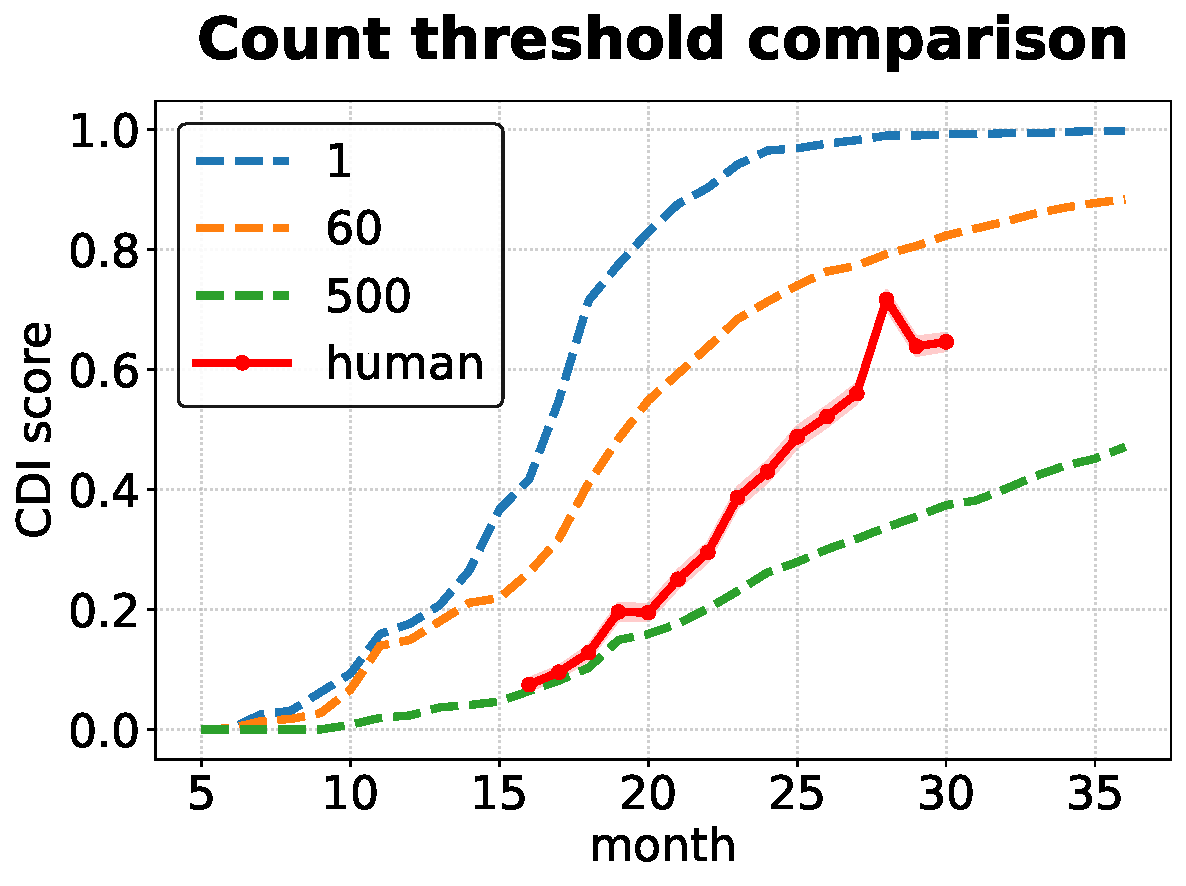
\includegraphics[width=0.5\textwidth]{fig/threshold.pdf}}
\caption{\textbf{Count-based calibration.} Child corpus vocabulary trajectories obtained with count thresholds of 1, 60, and 500, alongside the caregiver-report reference (red). The selected threshold of 60 is the calibration used in the main analysis. The curves illustrate the sensitivity of coverage and trajectory to the count criterion; their comparison does not by itself validate equivalence to caregiver reports.}
\label{fig:threshold}
\end{figure}


The frequency-matched evaluation list and the finite generation budget introduce distinct sampling choices. Figure~\ref{fig:distr} examines the second choice beyond the selected list by comparing training and generation word counts for an LSTM trained on 3.4M words, with generation volumes of 1, 10, and 100 times the reference amount. Larger output samples reduce the proportion of training words that are never generated, including in the lower-frequency range, but some rare words remain absent. The bottom panel therefore shows how observed absence changes as the sampling budget increases for a fixed trained model by the model. Absolute generated counts also rise mechanically with sample size, so movement in the scatter plot cannot alone be interpreted as improved learning or better-normalized word frequencies.


\begin{figure}[ht]
\centering
\subfloat{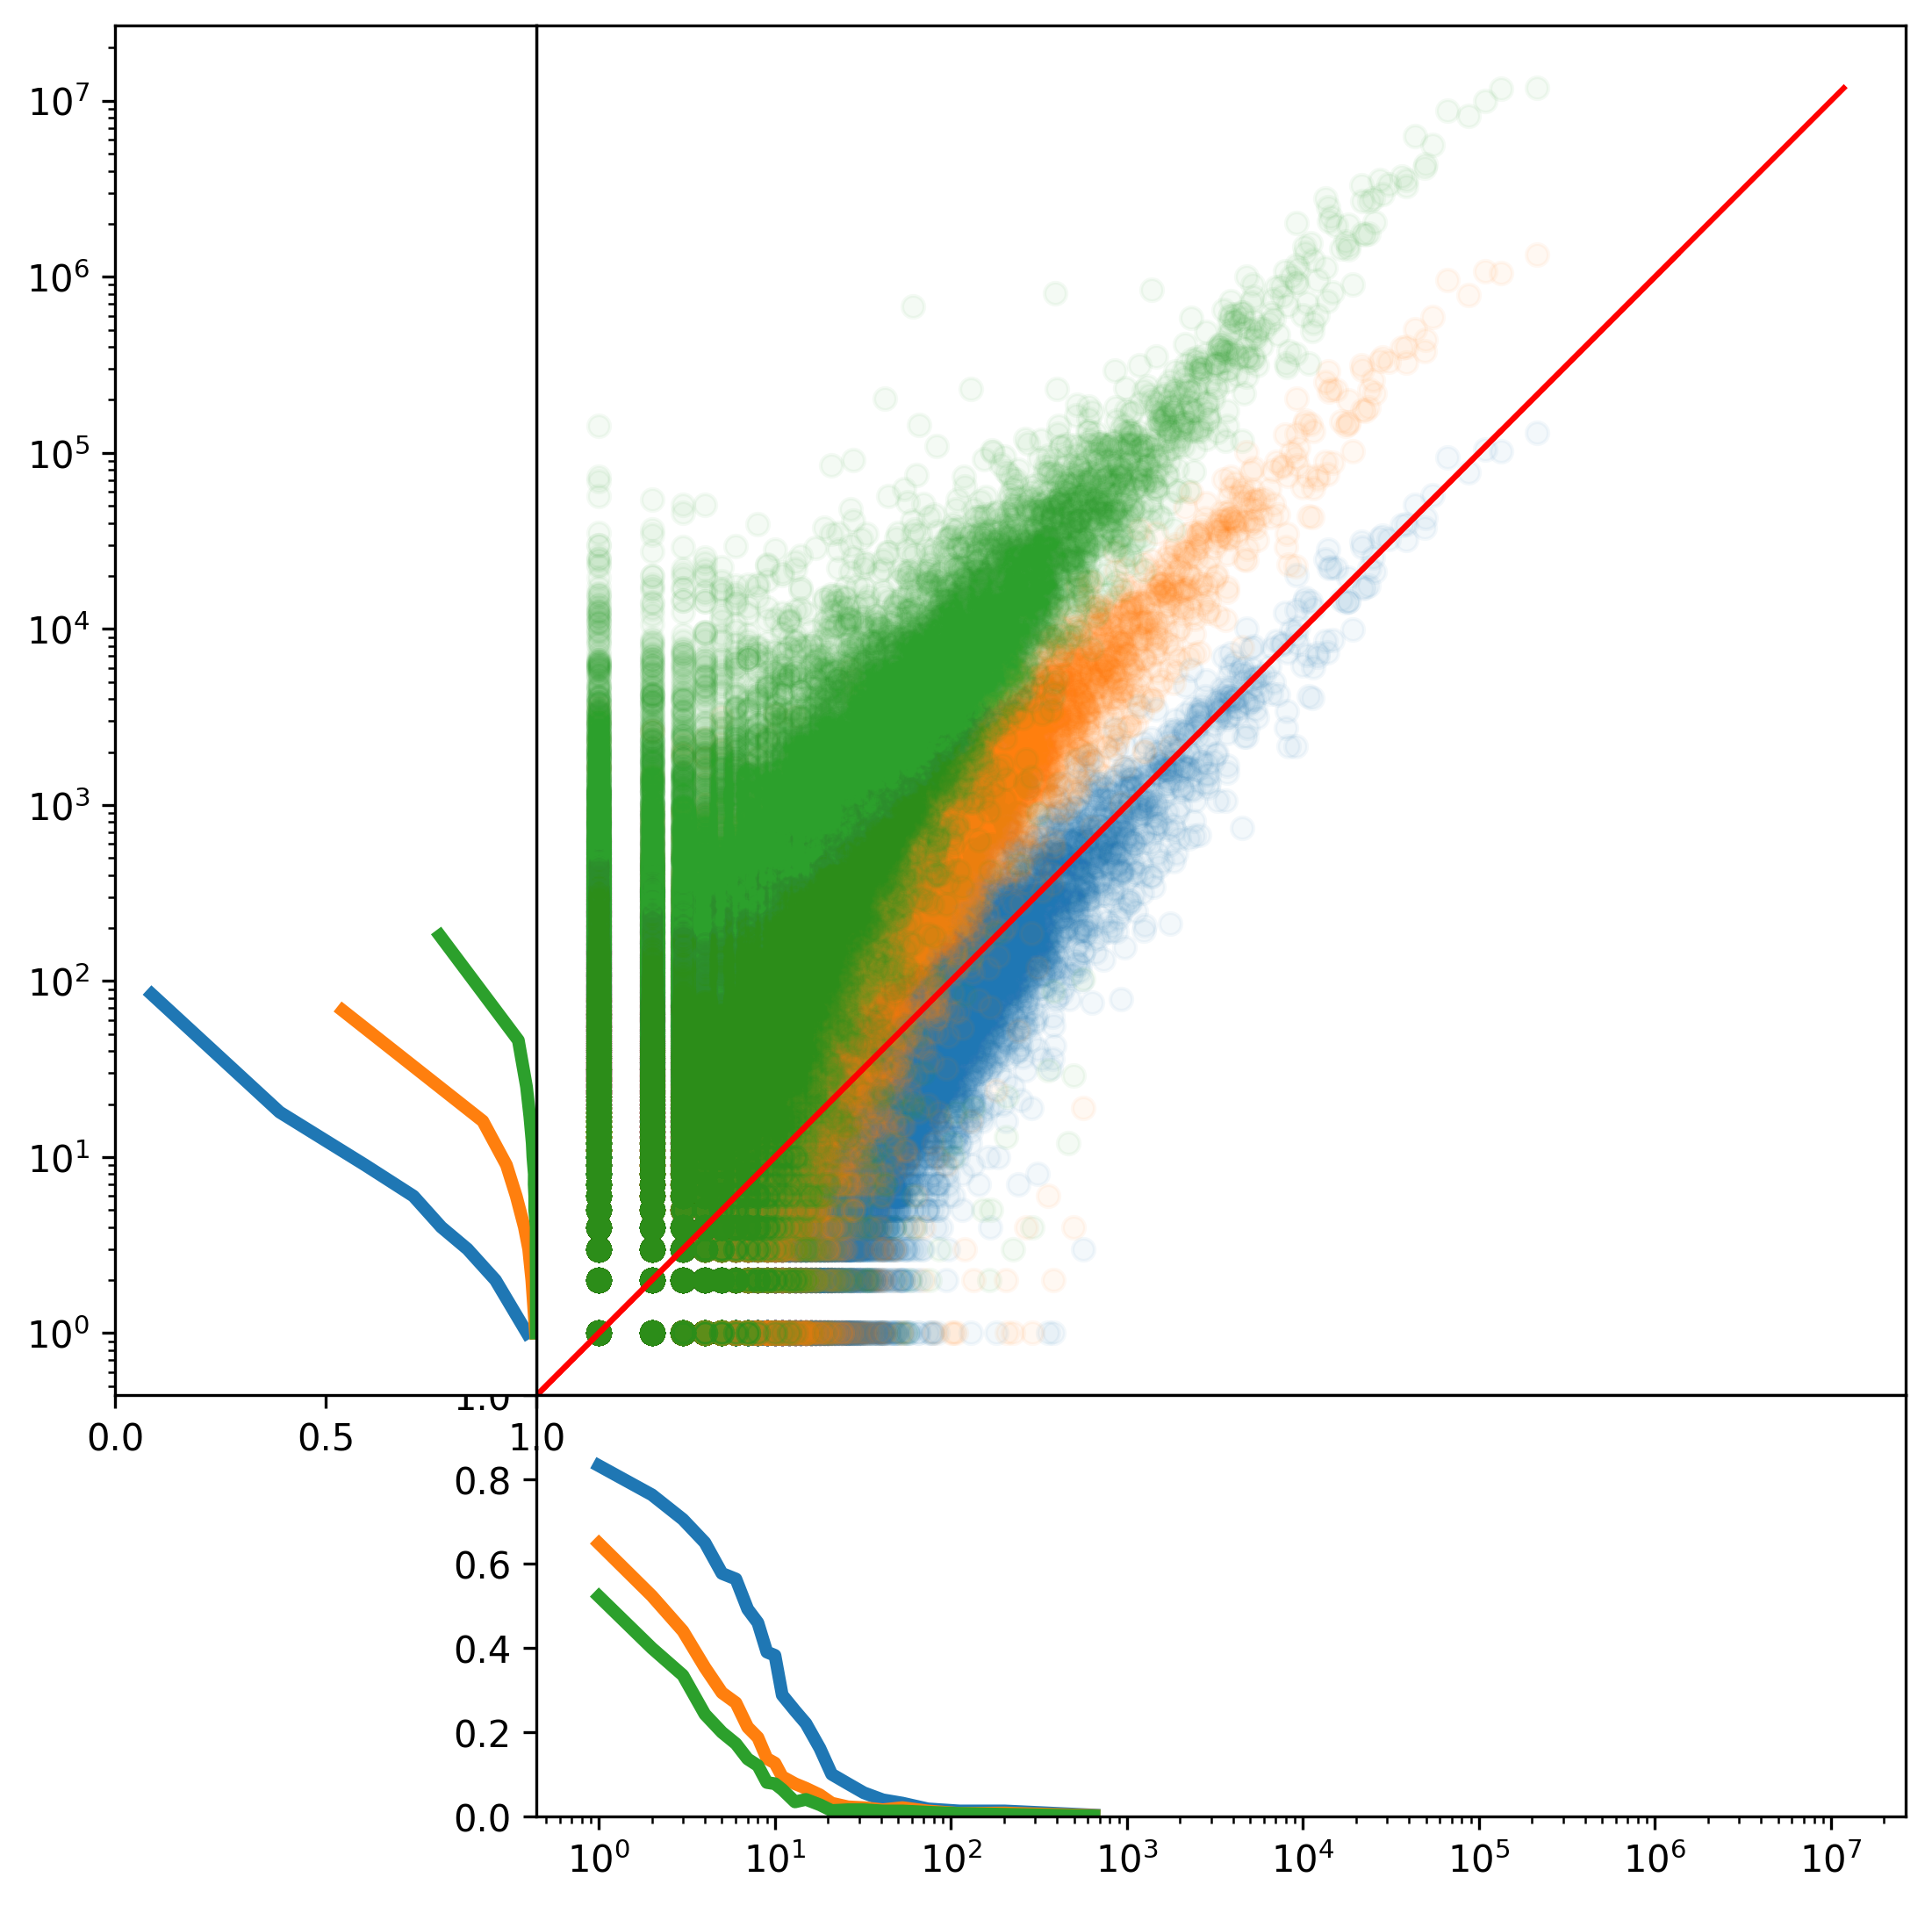
\includegraphics[width=0.3\textwidth]{fig/distr_LSTM_400.png}}
\hspace{1 pt}
\subfloat{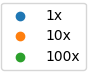
\includegraphics[width=0.1\textwidth]{fig/distr_cap.png}}
\caption{\textbf{Word count distribution(temperature = 1.0)}.Word frequency relationships between training and generation sets under different sampling conditions (1x, 10x, 100x generation volume). x-axis: word frequency in the training set; y-axis: word frequency in the generation set. The bottom panel shows the proportion of training word types absent from generated output as a function of their training count.}
\label{fig:distr}
\end{figure}


The exposure-scaling analysis in Figure~\ref{fig:hour} compares \meCDI{} trajectories under three estimated annual input budgets. Larger input budgets improve coverage in some conditions but do not reproduce the child reference trajectory within the tested protocol. This is evidence about the effect of the tested corpus-size manipulation, not identification of a unique learning mechanism responsible for the discrepancy.

\begin{figure}[ht]
\centering
\subfloat{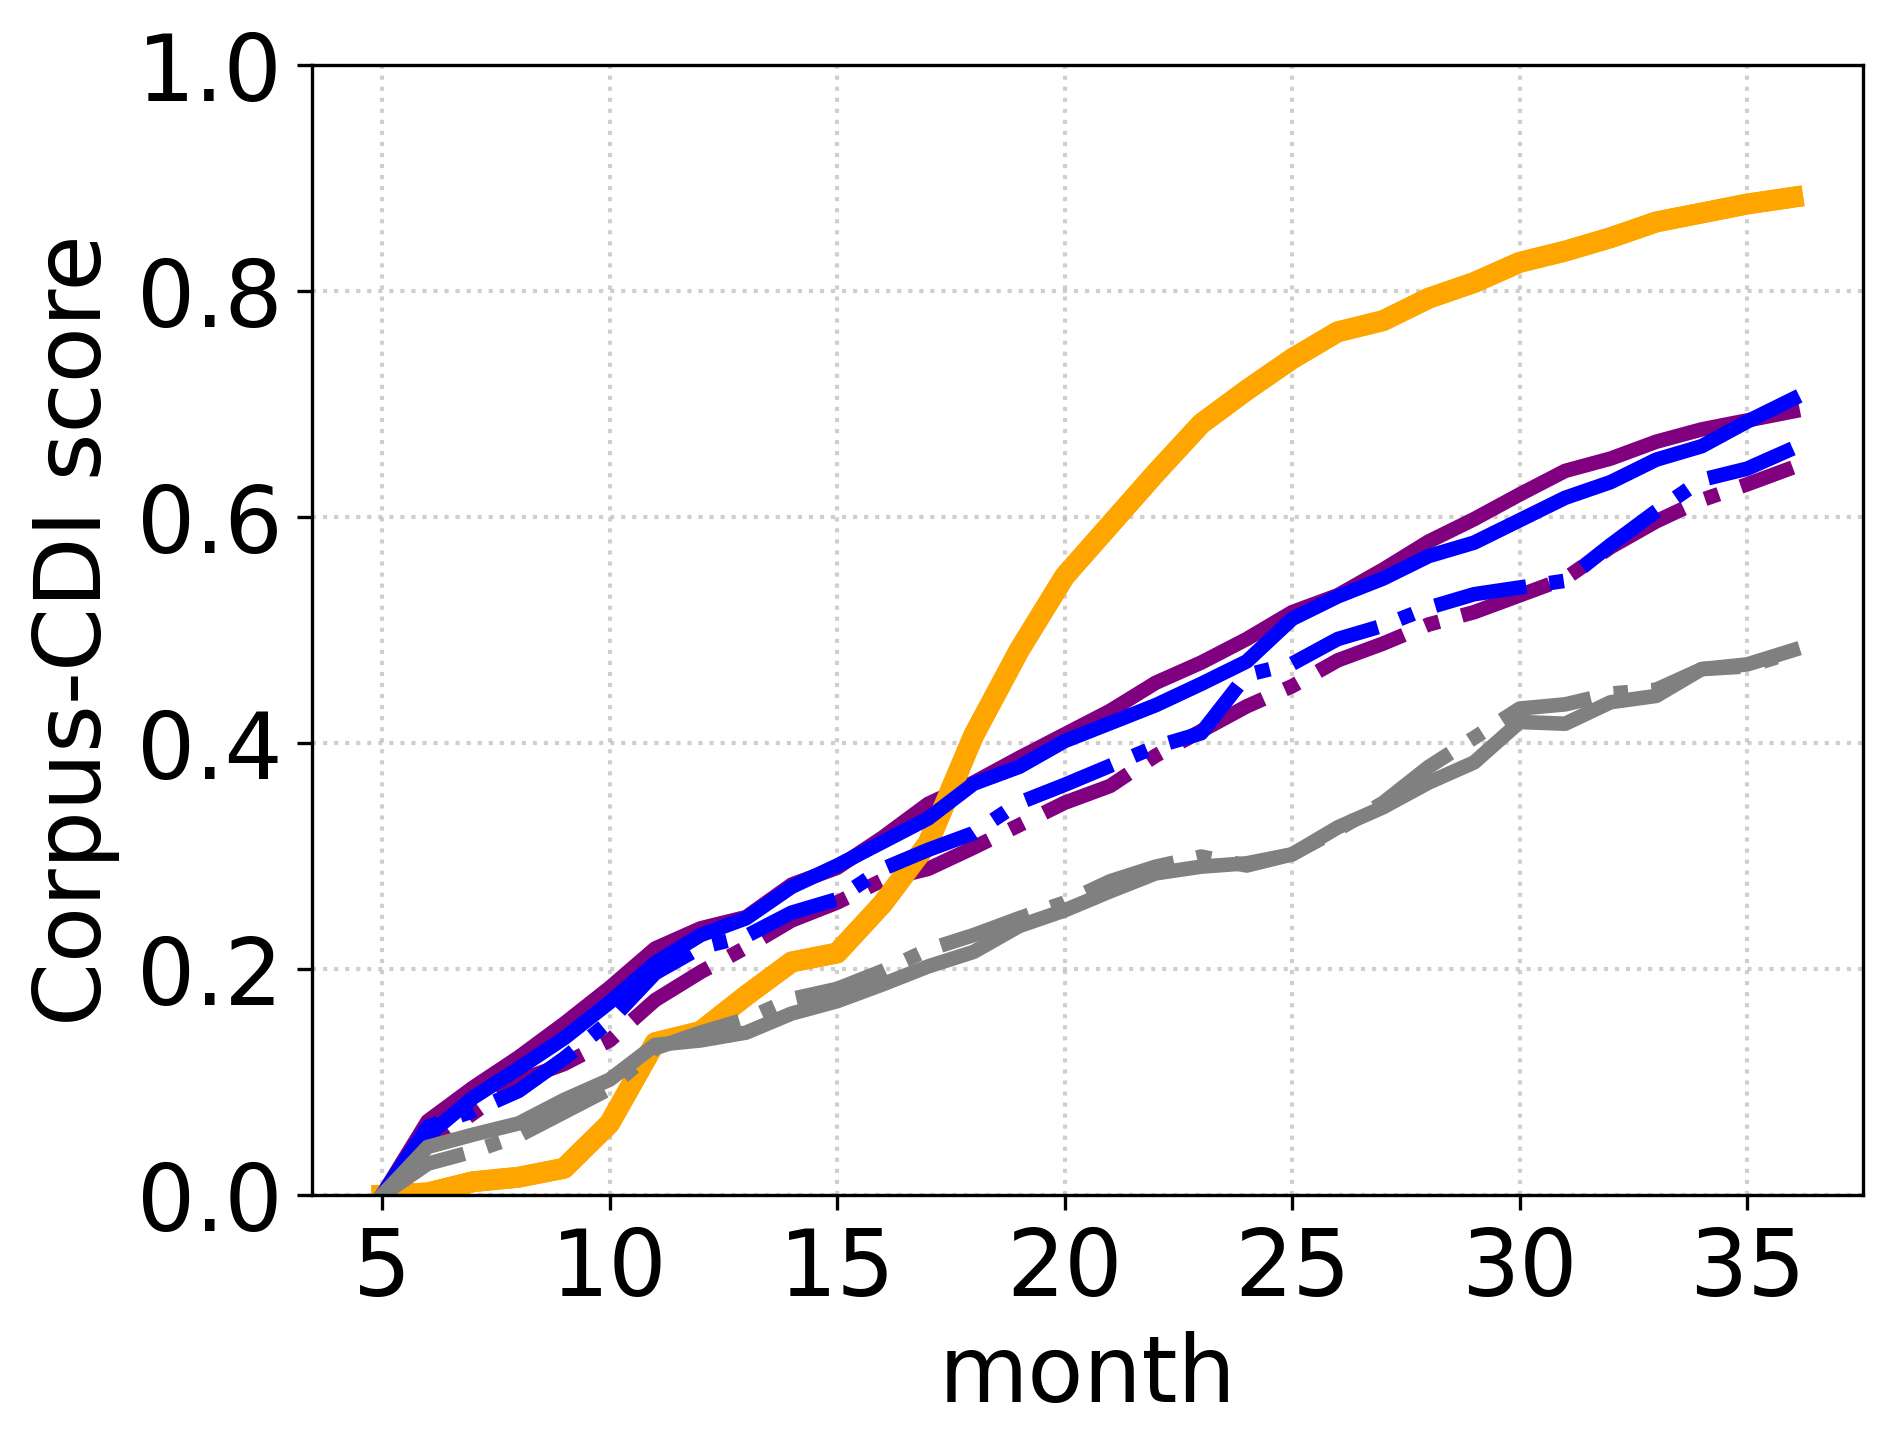
\includegraphics[width=0.35\textwidth]{fig/hour.png}}
\subfloat{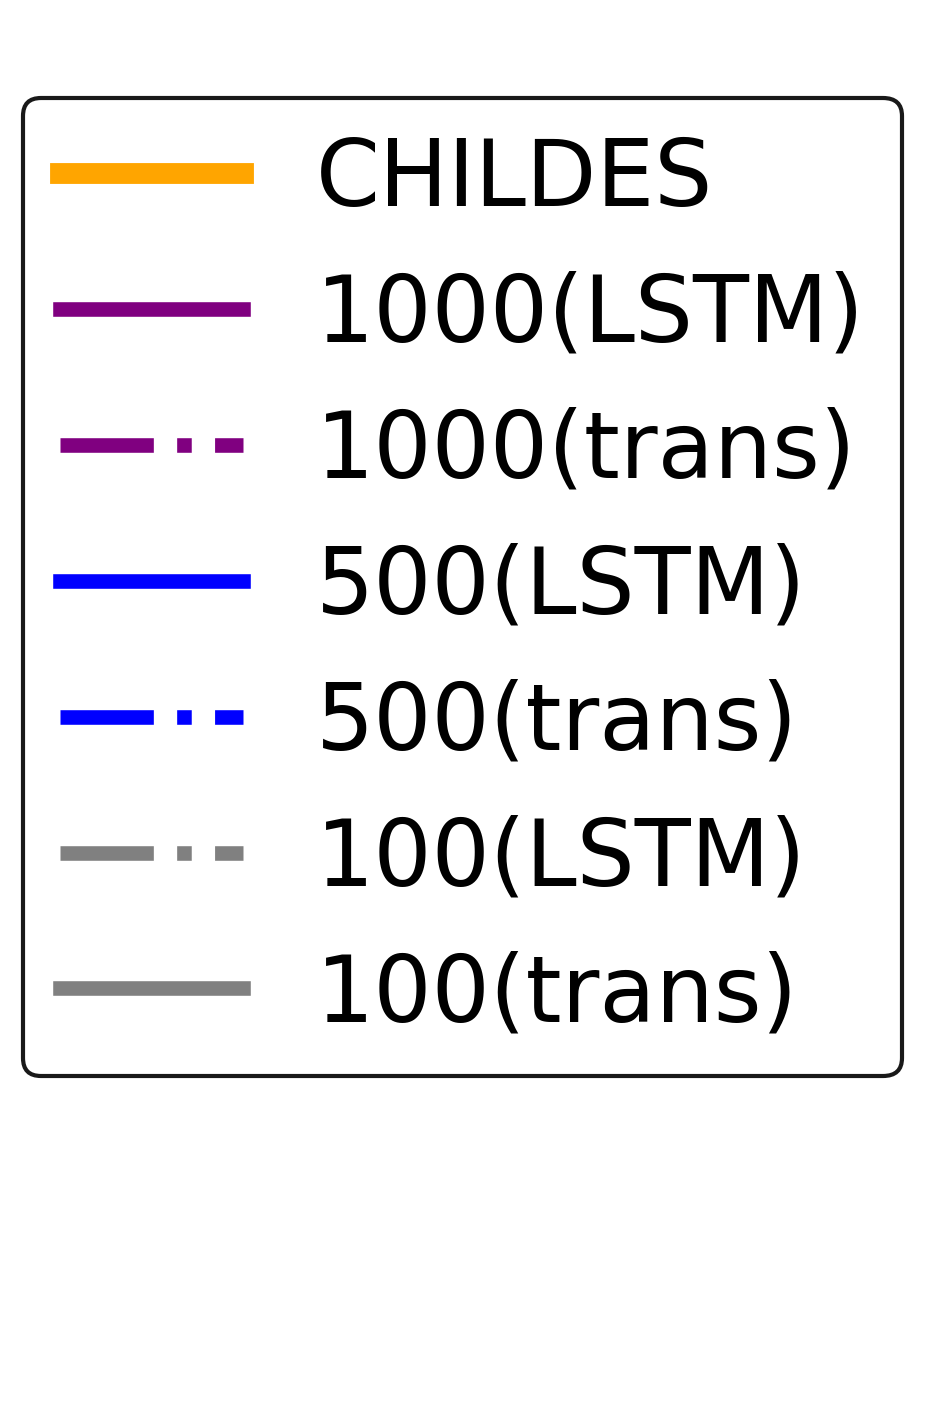
\includegraphics[width=0.1\textwidth]{fig/hour_legend.png}}
\caption{\textbf{Model vocabulary growth across estimated annual exposure levels.} Comparison of \meCDI{} trajectories for models trained on 100-, 500-, and 1000-hour exposure estimates, alongside CHILDES child production data. Models show roughly linear vocabulary growth that scales modestly with total exposure but remains far below the human developmental curve. }
\label{fig:hour}
\end{figure}

\clearpage
\endgroup
